\documentclass[10pt,xcolor=table, aspectratio=1610]{beamer}
% \special{dvipdfmx:config z 0}
\usetheme[progressbar=frametitle]{metropolis}

\usepackage[english]{babel}
\usepackage[export]{adjustbox}
\usepackage[outputdir=out]{minted}
\usemintedstyle{monokai}
\definecolor{LightGray}{HTML}{1f1f1f}
\usepackage{appendixnumberbeamer}
\usepackage{booktabs}
\usepackage{ellipsis}
\usepackage{csquotes}
\usepackage{hhline}
\usepackage{textgreek}
\usepackage{url}
\def\UrlBreaks{\do\/\do-}

\usepackage{caption}
\captionsetup{justification   = raggedright,
              singlelinecheck = off,
              font=scriptsize,
              labelfont=scriptsize}
\setlength{\abovecaptionskip}{2pt}
\setlength{\belowcaptionskip}{0pt}


\setbeamertemplate{footline}{
  \begin{beamercolorbox}{footer nav}
    \vskip 2pt \insertnavigation{\paperwidth} \vskip 2pt
  \end{beamercolorbox}
}

\newcommand{\supercite}[1]{\textsuperscript{\cite{#1}}}
\newcommand{\supercitepage}[2][]{\textsuperscript{\cite[#1]{#2}}}

\title{Diagrammatic Monte Carlo}
\subtitle{Exercises}
\date{\today}
\author{Jonas Märtens}
\institute{University of Bologna}

\begin{document}
\maketitle

\begin{frame}[containsverbatim]{Contents}
  \setbeamertemplate{section in toc}[sections numbered]
  \tableofcontents%[hideallsubsections]
\end{frame}

\section{Task 1: Monte Carlo Basics - Estimating PI}

\begin{frame}[containsverbatim]{Estimating PI - Task}
\begin{columns}
        \column{0.5\linewidth}
          Two different methods to estimate $\pi$:
          \begin{itemize}
            \item \alert{Area Method} (as seen in the picture)
            \item \alert{MC Integration Method}
                  $\pi/4=\int_0^1\sqrt{1-x^2}dx=\int_0^1\frac{\sqrt{1-x^2}}{p(x)}p(x)dx=\langle \frac{\sqrt{1-x^2}}{p(x)}\rangle_p\approx\frac{1}{N}\sum_{i=1}^{N}\frac{\sqrt{1-x_i^2}}{p(x_i)}$
                  for $p(x)=1$ and $x_i\sim U(0,1)$
          \end{itemize}
        \column{0.5\linewidth}
          \begin{figure}
            \centering
            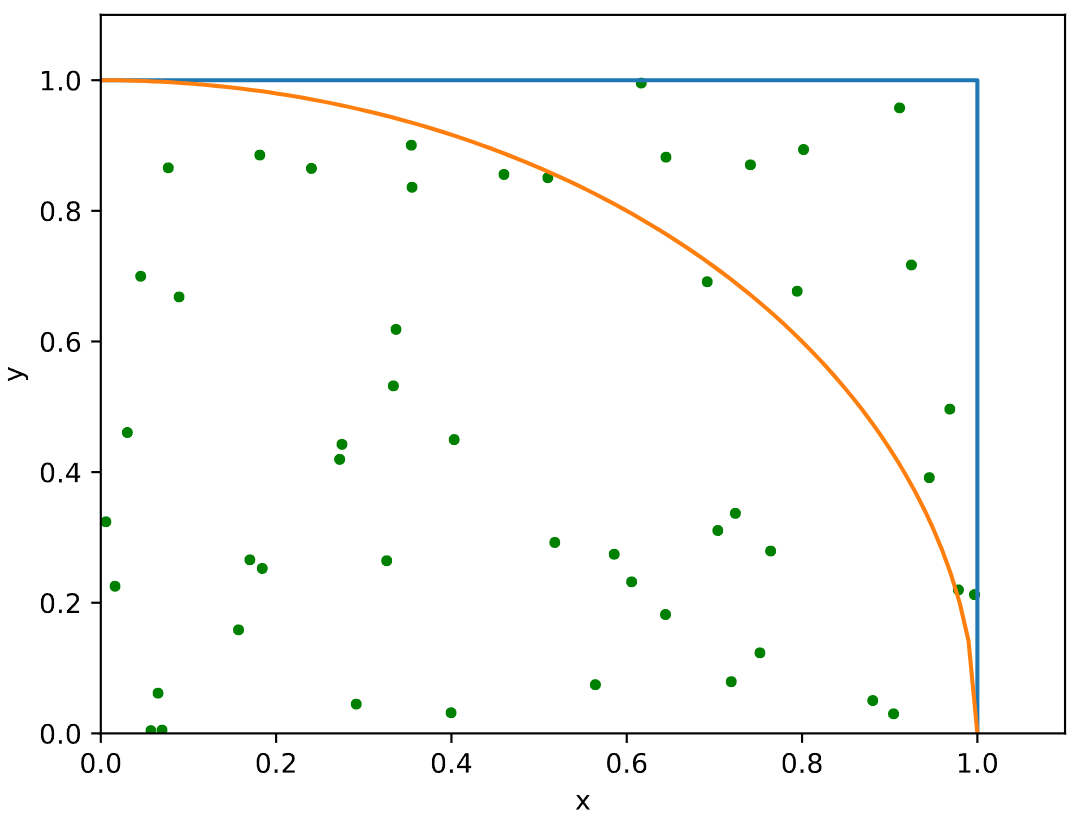
\includegraphics[width=\linewidth]{images/area_method_visualization.png}
            \caption{Visualization of the area method.\cite{tasks}}
          \end{figure}
\end{columns}
\end{frame}

\begin{frame}[containsverbatim]{Estimating PI: Area Method - Implementation}
  \begin{minted}
    [
      baselinestretch=1.2,
      bgcolor=LightGray,
      fontsize=\scriptsize,
      linenos
      ]
      {python}
def area_method(n, plot=False):
    n_in = 0
    estimates_n = np.array([], dtype=int)
    estimates_area = np.array([])
    for i in range(n):
        # generate random numbers between 0 and 1
        x = np.random.random()
        y = np.random.random()
        # check if the point is in the circle
        if x**2 + y**2 <= 1:
            n_in += 1
        # every 10000 points, calculate the area
        if plot:
            if i % (int(n / 100000)) == 0 and i > 1000000:
                estimates_n = np.append(estimates_n, i + 1)
                estimates_area = np.append(estimates_area, 4 * n_in / (i + 1))
    if plot:
        # Do the plotting here
        # ...
    return 4 * n_in / n
  \end{minted}
\end{frame}

\begin{frame}[containsverbatim]{Estimating PI: Area Method - Convergence}
  \begin{minted}
    [
      baselinestretch=1.2,
      bgcolor=LightGray,
      fontsize=\footnotesize,
      linenos
      ]
      {python}
area_method(int(1e8), plot=True)
  \end{minted}
  \begin{figure}
    \centering
    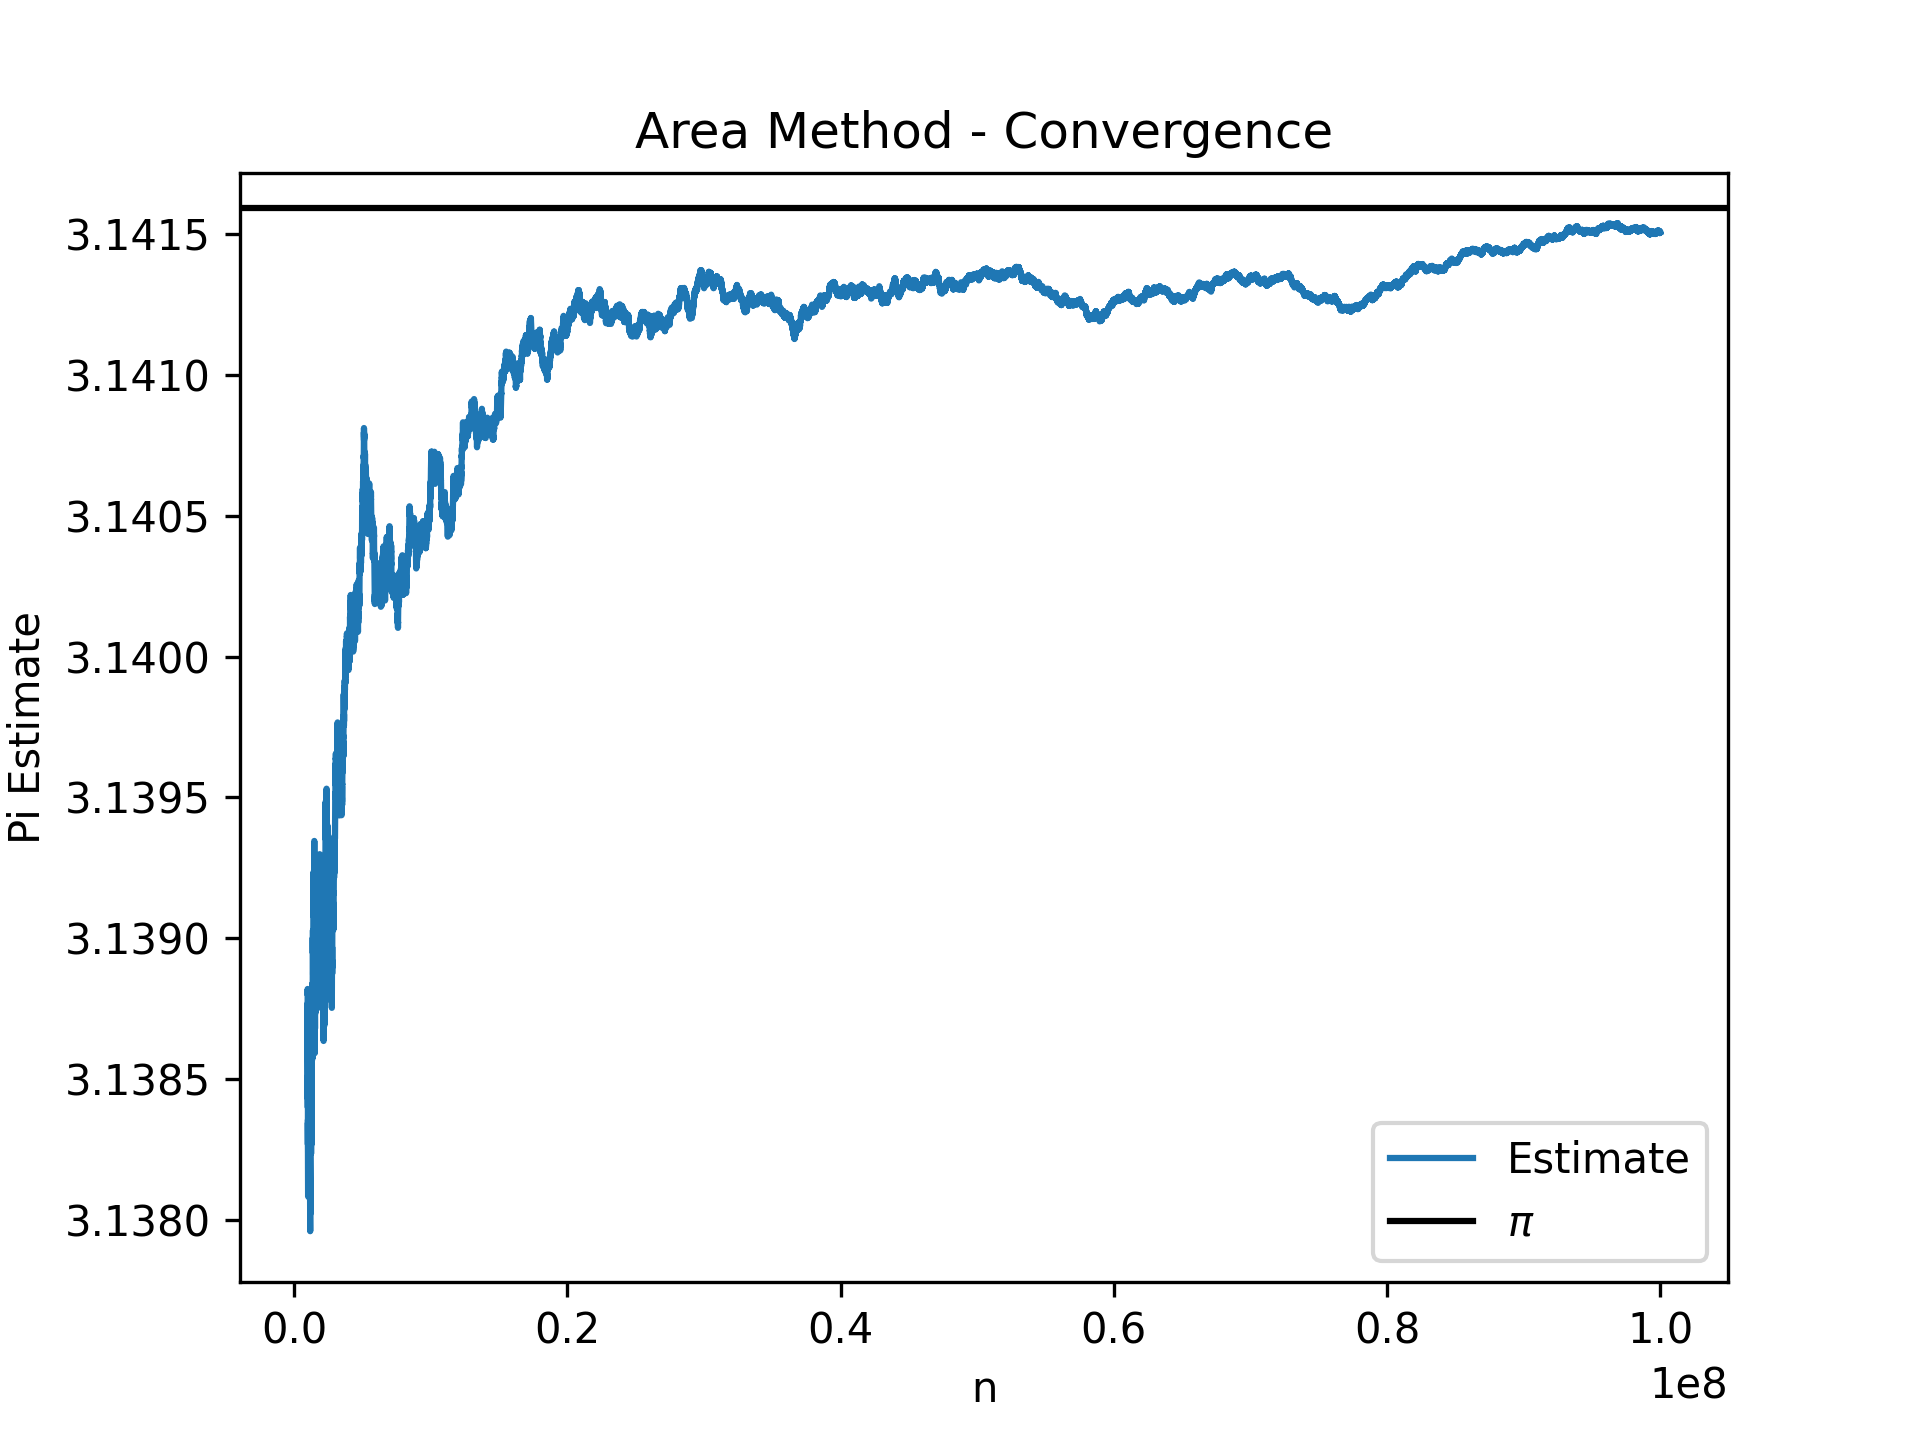
\includegraphics[width=0.65\textwidth]{images/area_method_convergence2.png}
  \end{figure}
\end{frame}

\begin{frame}[containsverbatim]{Estimating PI: Area Method - We can do better}
  \begin{minted}
    [
      baselinestretch=1.2,
      bgcolor=LightGray,
      fontsize=\footnotesize,
      linenos
      ]
      {python}
def area_method_fast(n):
    x = np.random.random(n)
    y = np.random.random(n)
    n_in = np.sum(x**2 + y**2 <= 1)
    return 4 * n_in / n
  \end{minted}
  \begin{minted}
    [
      baselinestretch=1.2,
      bgcolor=LightGray,
      fontsize=\footnotesize,
      linenos
      ]
      {python}
pis = np.zeros(10000)
for i in range(10000):
    pis[i] = area_method_fast(int(1e6))
std = np.std(pis)
mean = np.mean(pis)
# Do the plotting here
# ...
print("Area Method:")
print(f"{mean = }")
print(f"{std = }")
  \end{minted}
  
\end{frame}

\begin{frame}[containsverbatim]{Estimating PI: Area Method - Histogram}
  \begin{figure}
    \centering
    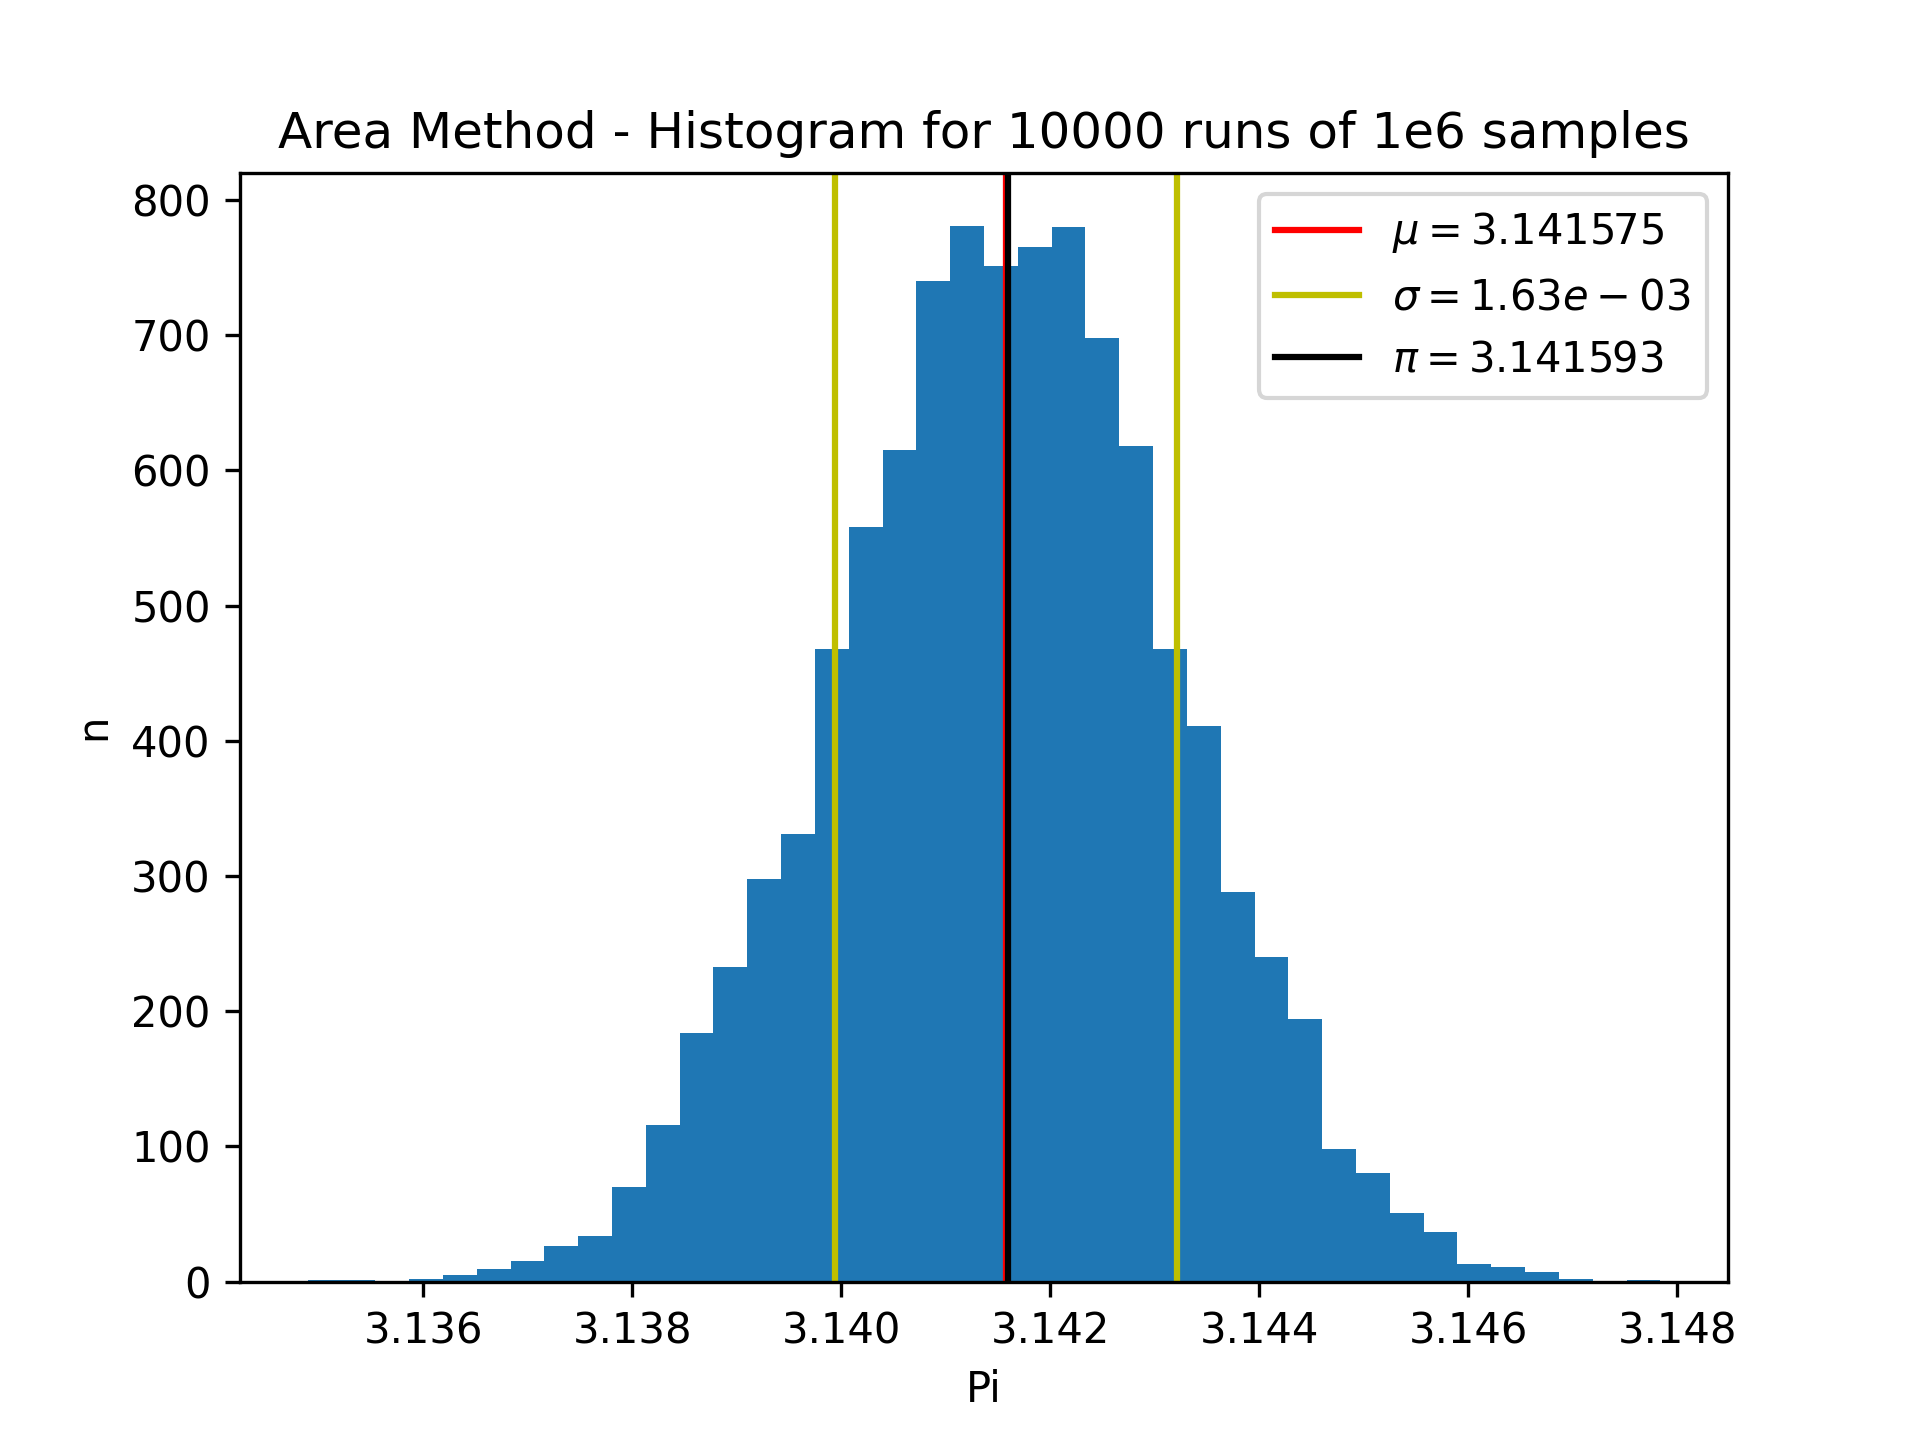
\includegraphics[width=0.8\textwidth]{images/area_method_histogram2.png}
  \end{figure}
\end{frame}


\begin{frame}[containsverbatim]{Estimating PI: MC Integration Method - Implementation}
  \begin{minted}
    [
      baselinestretch=1.2,
      bgcolor=LightGray,
      fontsize=\footnotesize,
      linenos
      ]
      {python}
def p(x):
    return 1

def f(x):
    return np.sqrt(1 - x**2)

def mc_integrate(n, plot=False):
    sum = 0
    estimates_n = np.array([], dtype=int)
    estimates_area = np.array([], dtype=np.float32)
    for i in range(n):
        x = np.random.random()
        sum += f(x) / p(x)
        if plot and i % (int(n / 100000)) == 0 and i > 1000000:
            estimates_n = np.append(estimates_n, i+1)
            estimates_area = np.append(estimates_area, 4 * sum / (i+1))
    if plot:
        # Do the plotting here
    return sum / n * 4
  \end{minted}
  
\end{frame}

\begin{frame}[containsverbatim]{Estimating PI: MC Integration Method - Convergence}
  \begin{minted}
    [
      baselinestretch=1.2,
      bgcolor=LightGray,
      fontsize=\footnotesize,
      linenos
      ]
      {python}
mc_integrate(int(1e8), plot=True)
  \end{minted}
  \begin{figure}
    \centering
    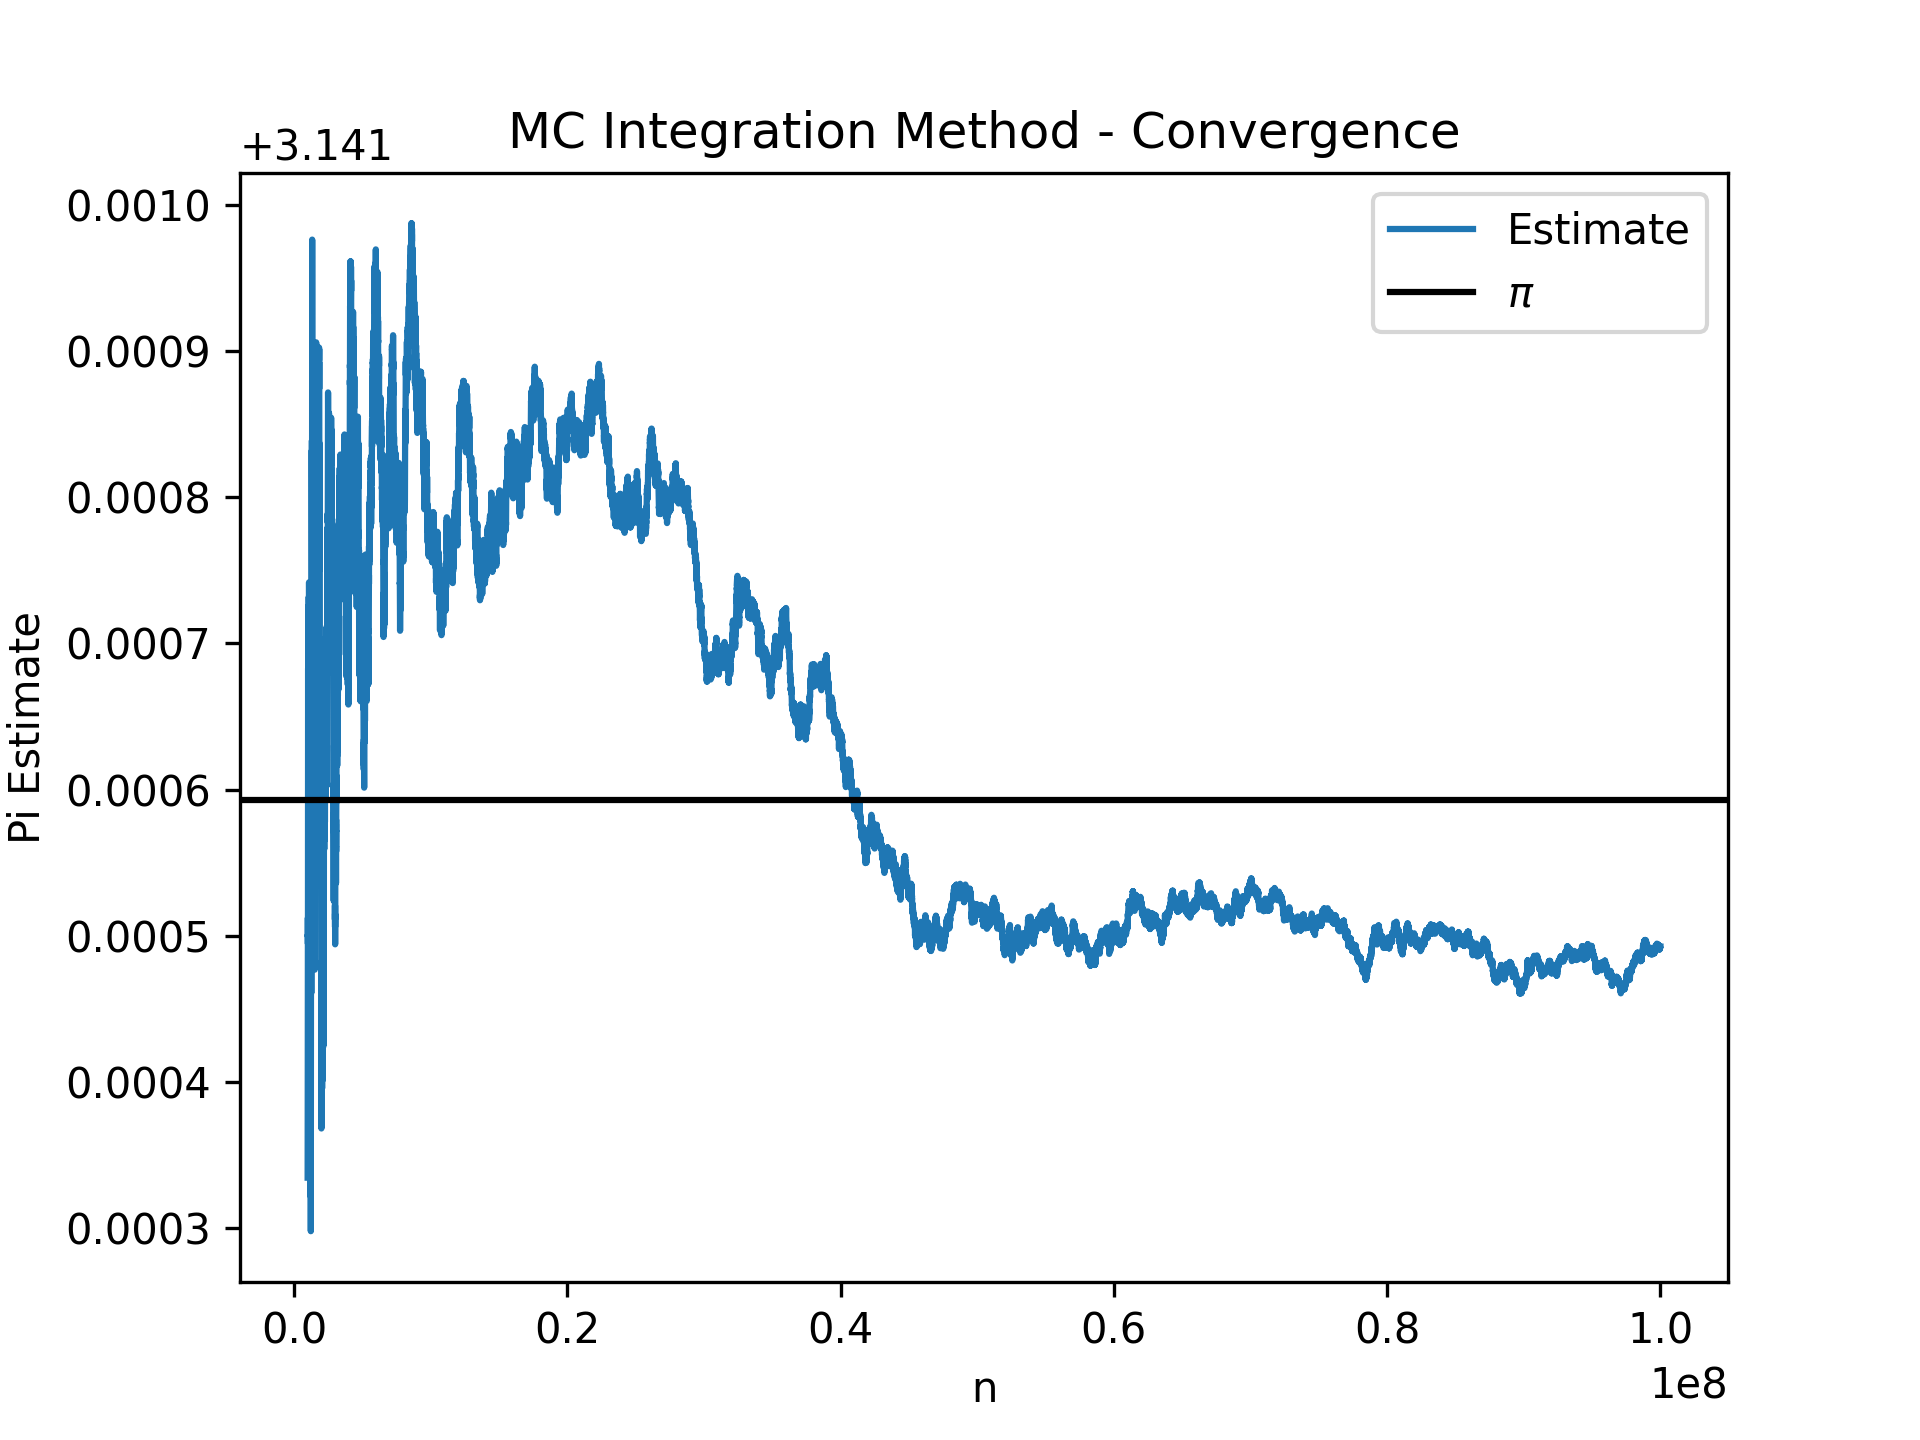
\includegraphics[width=0.65\textwidth]{images/mc_integration_method_convergence2.png}
  \end{figure}
\end{frame}

\begin{frame}[containsverbatim]{Estimating PI: MC Integration Method - We can do better}
  \begin{minted}
    [
      baselinestretch=1.2,
      bgcolor=LightGray,
      fontsize=\footnotesize,
      linenos
      ]
      {python}
def mc_integrate_fast(n):
    x = np.random.random(n)
    return np.sum(f(x)) / n * 4
  \end{minted}
  \begin{minted}
    [
      baselinestretch=1.2,
      bgcolor=LightGray,
      fontsize=\footnotesize,
      linenos
      ]
      {python}
pis = np.zeros(10000)
for i in range(10000):
    pis[i] = mc_integrate_fast(int(1e6))
std = np.std(pis)
mean = np.mean(pis)
# Do the plotting here
# ...
print("MC Integration Method:")
print(f"{mean = }")
print(f"{std = }")
  \end{minted}
  
\end{frame}

\begin{frame}[containsverbatim]{Estimating PI: Area Method - Histogram}
  \begin{figure}
    \centering
    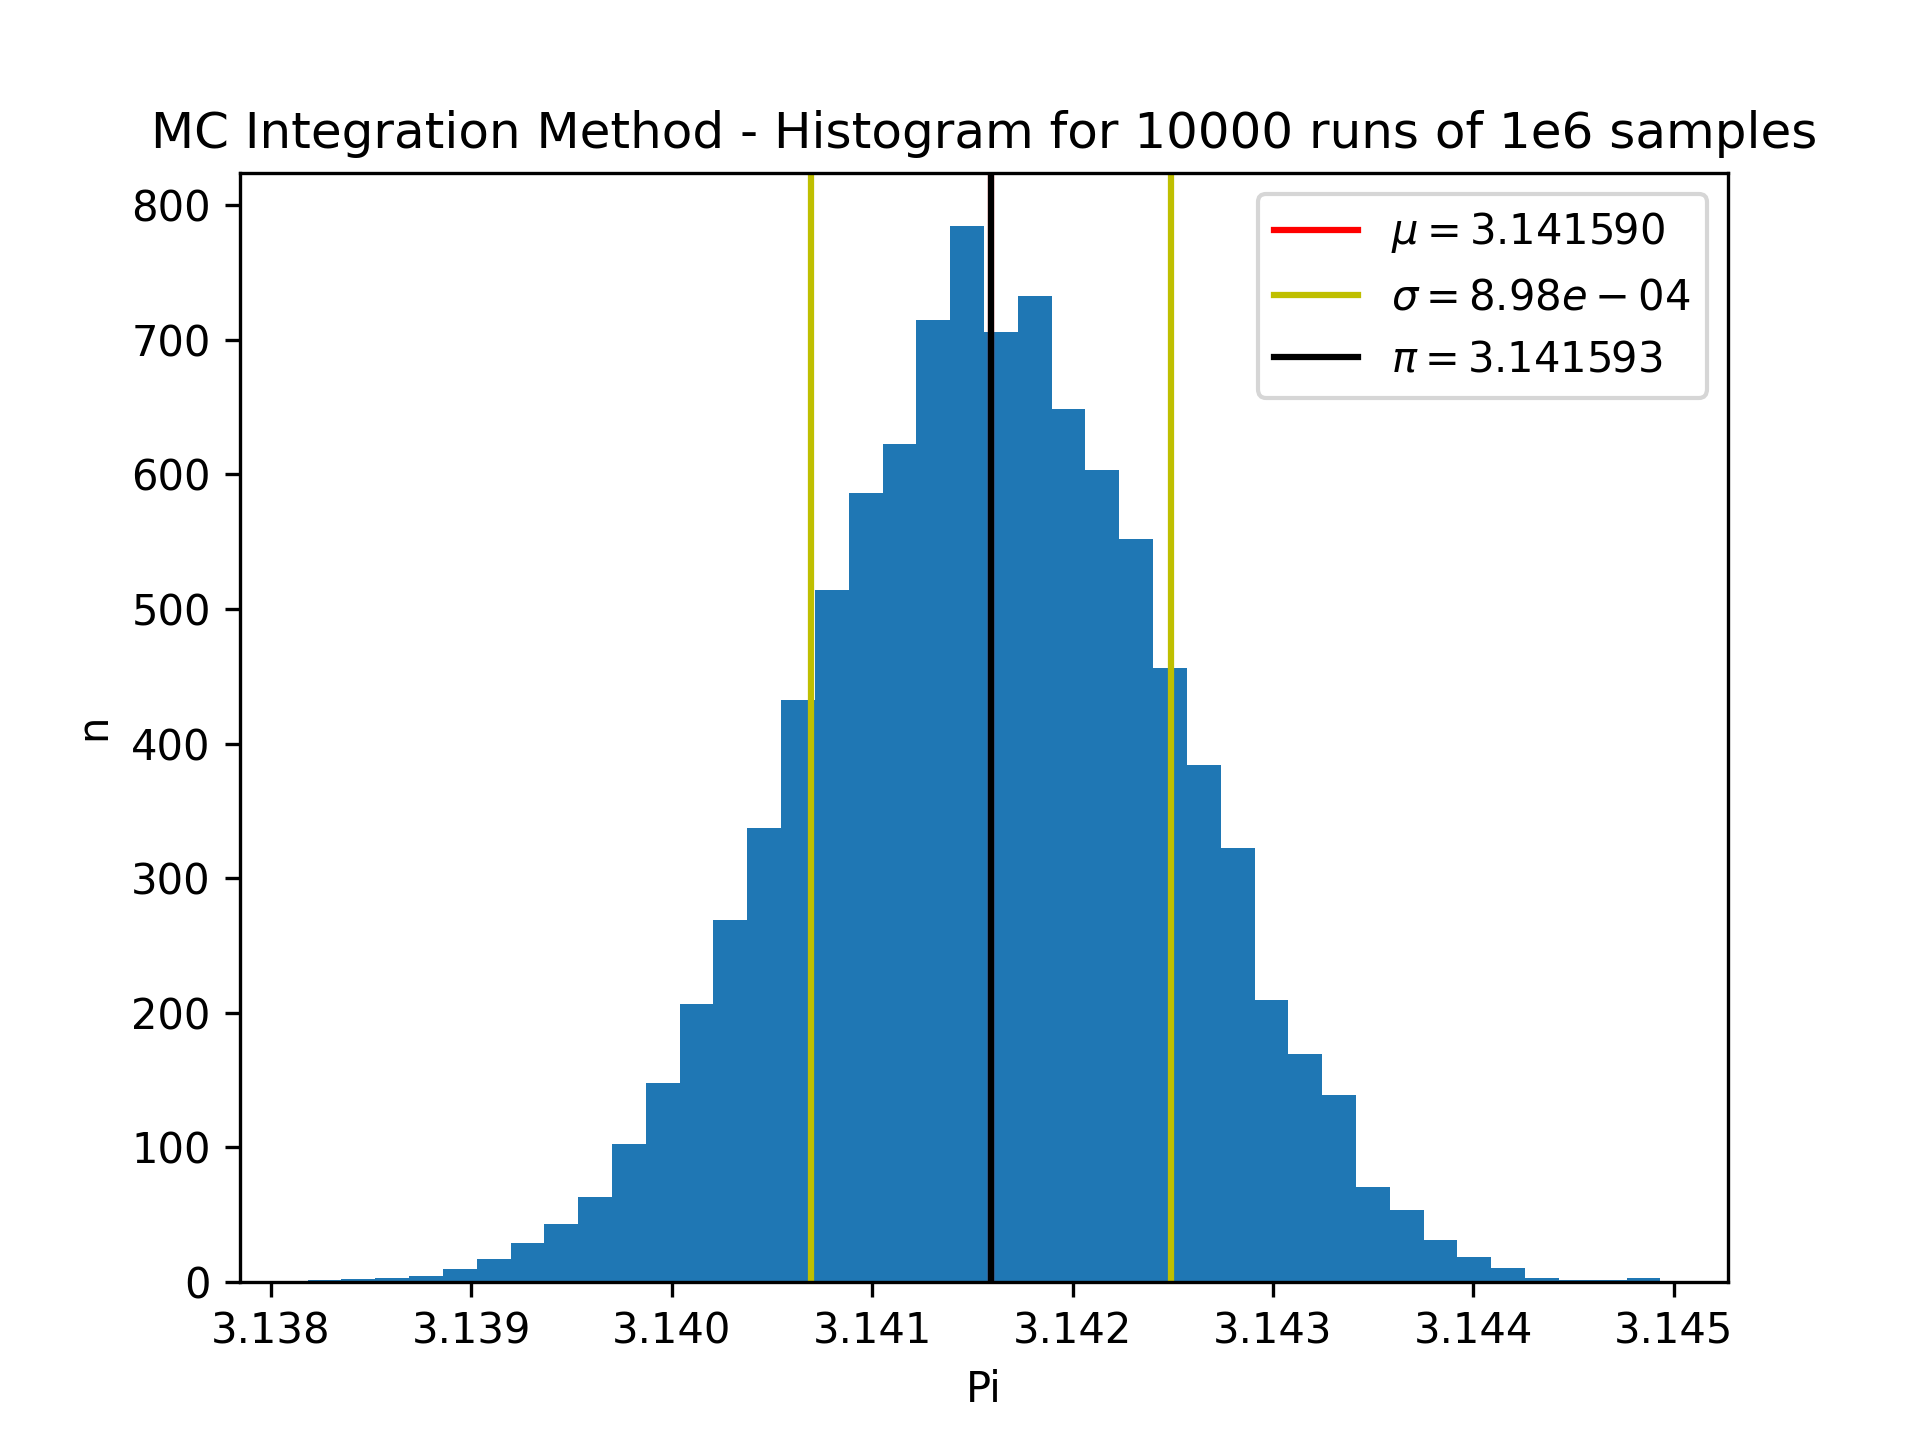
\includegraphics[width=0.8\textwidth]{images/mc_integration_method_histogram2.png}
  \end{figure}
\end{frame}

\section{Task 2: CDF Inversion}
\begin{frame}[containsverbatim]{CDF Inversion - Task}
  Let $Q(\tau,\alpha)=\exp(-\alpha\tau)$. and
  $F(\tau) = \frac{1 - \exp(-\alpha \tau)}{\alpha}$ the CDF. Sample from $Q$ by
  inverting:
  \begin{equation*}
    r=\frac{\int_{\tau_{\min }}^\tau Q\left(\tau^{\prime}\right) d \tau^{\prime}}{\int_{\tau_{\min }}^{\tau_{\max }} Q\left(\tau^{\prime}\right) d \tau^{\prime}}=\frac{F(\tau)-F\left(\tau_{\min }\right)}{F\left(\tau_{\max }\right)-F\left(\tau_{\min }\right)}
  \end{equation*}
  with $r\sim U(0,1)$. Setting $\tau_{\min}=0$ and $\tau_{\max}=5$ and solving:
  \begin{equation*}
    \tau = -\frac{\log(1 - \alpha\cdot r\cdot F(\tau_{\max}))}{\alpha}
  \end{equation*}

  We can now
  \begin{itemize}
    \item Sample from $Q$ and plot the histogram
    \item Calculate $I_1=\int_0^5 \tau Q(\tau, \alpha) d \tau=\langle \tau\rangle\cdot \text{Norm}=\langle \tau\rangle\cdot F(\tau_{\max})$
    \item Calculate $I_2=\int_0^5 \tau^2 Q(\tau, \alpha) d \tau=\langle \tau^2\rangle\cdot F(\tau_{\max})$
    \item Calculate $\sigma(I_1)$ and $\sigma(I_2)$: $\sigma(\overline{\tau})=\frac{\sigma_\text{Samples}}{\sqrt{n}}$\cite[p.47]{gubernatis}
  \end{itemize}
\end{frame}

\begin{frame}[containsverbatim]{CDF Inversion - Implementation}
  \begin{minted}
    [
      baselinestretch=1.2,
      bgcolor=LightGray,
      fontsize=\scriptsize,
      linenos
      ]
      {python}
alpha = 1
x_max = 5
n = int(1e8)

def F(x):
    return (1 - np.exp(-alpha*x))/alpha

F_max = F(x_max)

def F_inv(r):
    return -np.log(1 - alpha*r*F_max)/alpha

#generate all samples at once using numpy
r = np.random.random(n)
x = F_inv(r)
# Do the plotting here
# Use np.histogram or plt.hist
print("I1 exact: 1-6*exp(-5) = 0.9595723")
print(f"I1 mean: { np.mean(x)*F_max:.6f}")
print(f"I1 std: {np.std(x)*F_max/np.sqrt(n):.3e}")
print("I2 exact: 2-37*exp(-5) = 1.750696")
print(f"I2 mean: {np.mean(x**2)*F_max:.6f}")
print(f"I2 std: {np.std(x**2)*F_max/np.sqrt(n):.3e}")
  \end{minted}
\end{frame}

\begin{frame}[containsverbatim]{CDF Inversion - Histogram}
  \begin{columns}
          \column{0.35\linewidth}
          Console Output:
            \begin{minted}
              [
                baselinestretch=1.2,
                bgcolor=LightGray,
                fontsize=\scriptsize,
                linenos
                ]
                {python}
I1 exact: 0.9595723
I1 mean:  0.959501
I1 std:   9.045e-05
I2 exact: 1.750696
I2 mean:  1.750502
I2 std:   3.205e-04
              \end{minted}
          \column{0.65\linewidth}
          \begin{figure}
            \centering
            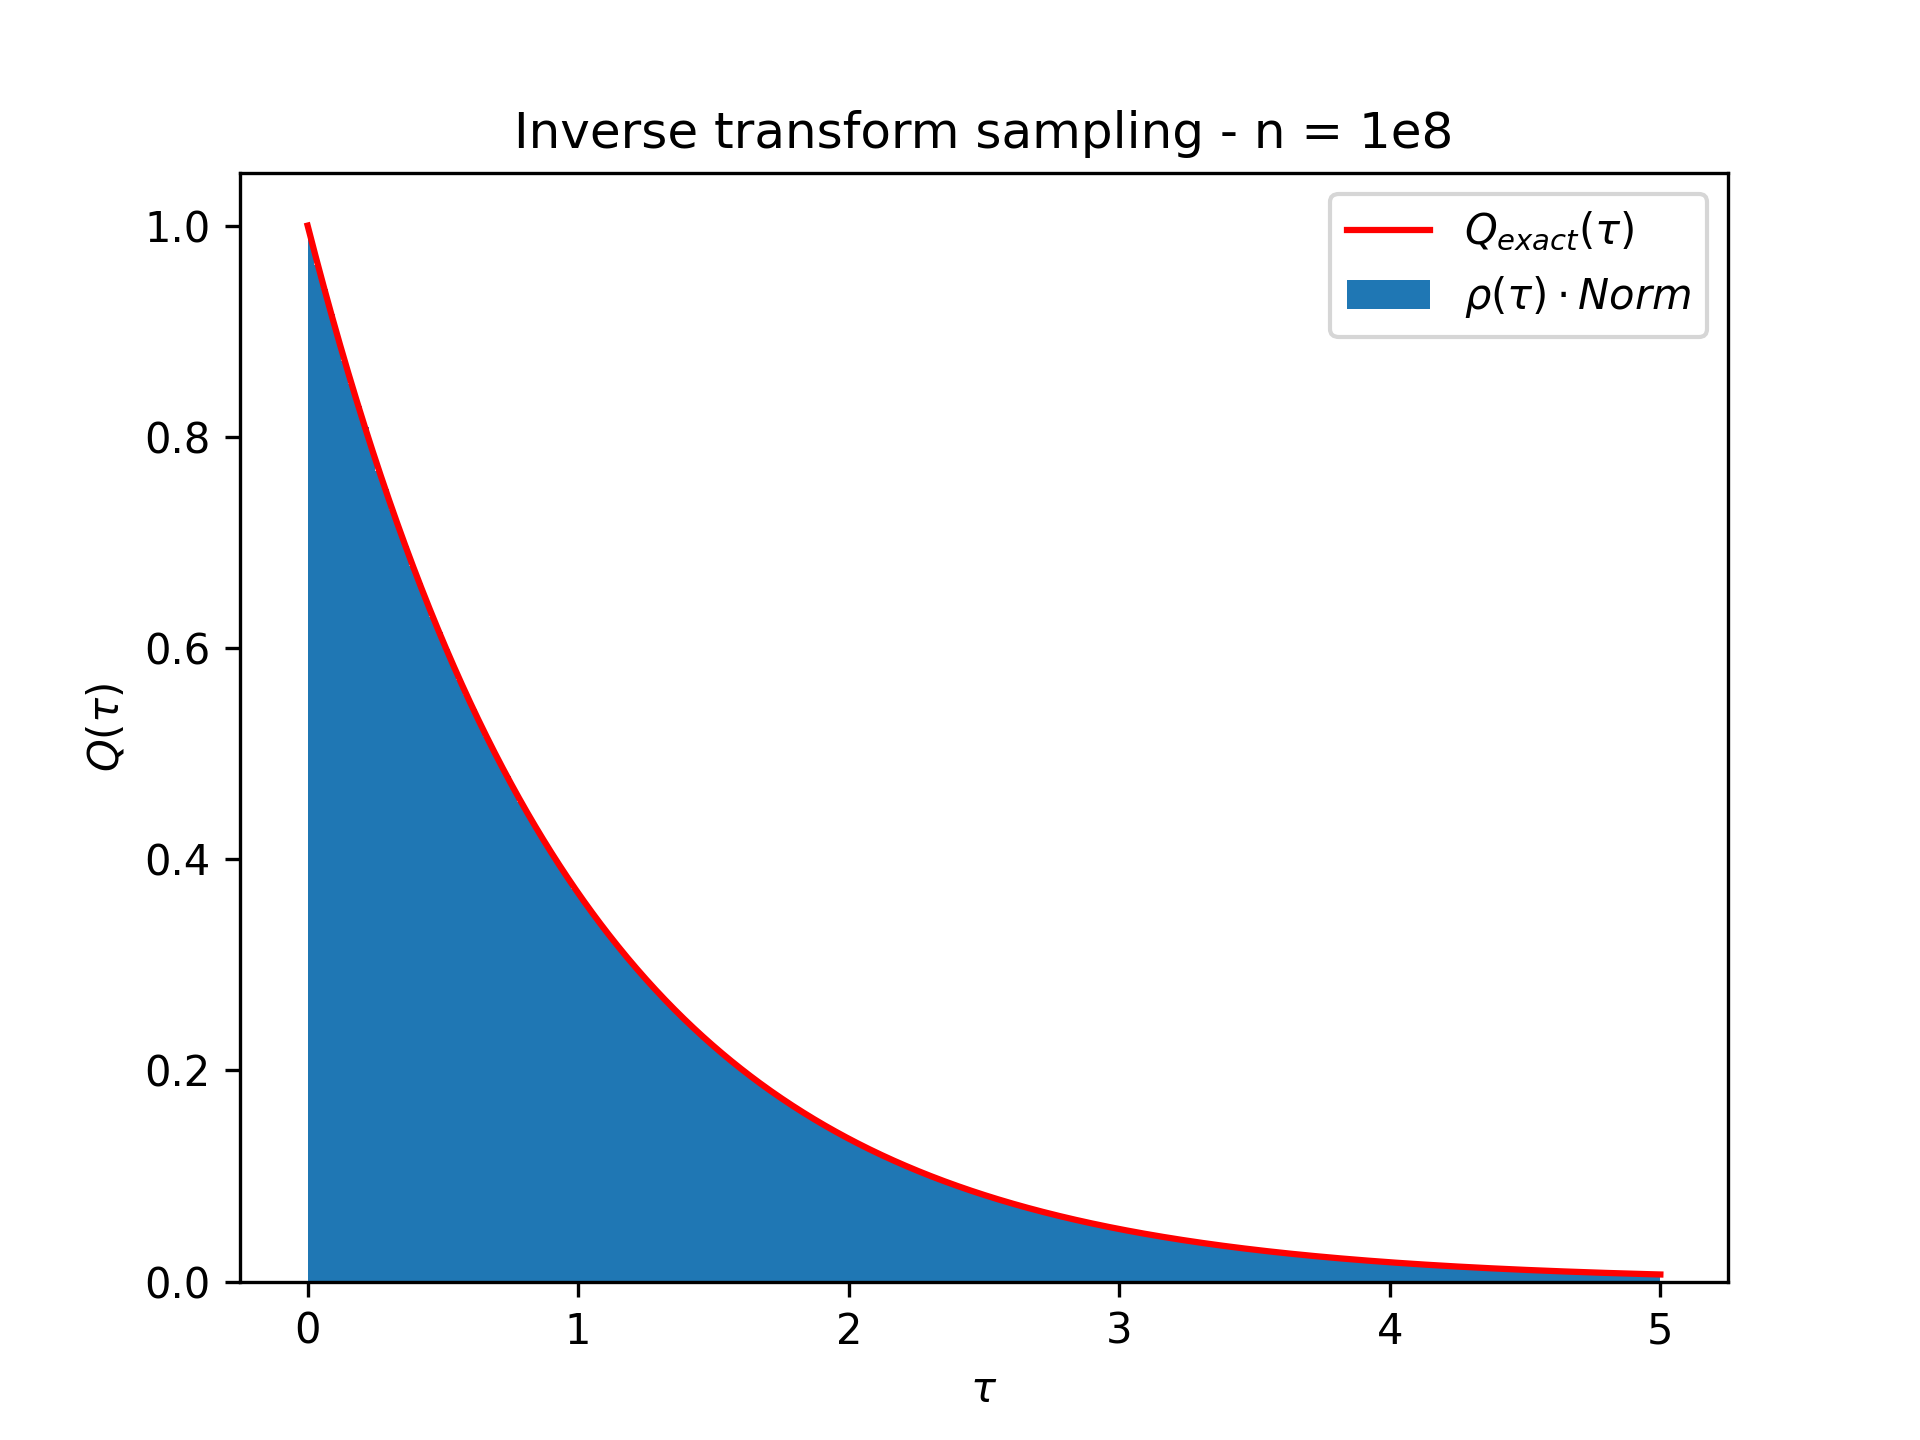
\includegraphics[width=\linewidth]{images/cdf_inversion2.png}
          \end{figure}
  \end{columns}
\end{frame}
  
\section{Task 3: Towards DMC - MCMC}

\begin{frame}[containsverbatim]{Markov Chain Monte Carlo - Task}
Basic principle behind DMC is Markov Chain Monte Carlo (MCMC). We again sample from
a distribution $f$, this time using the \alert{Metropolis-Hastings algorithm}:
\begin{itemize}
  \item Propose a random configuration $x^\prime$ from a proposal distribution $p$
  \item Accept the configuration with probability $A(x, x')=\min \left(1, \frac{f(x^{\prime}) p\left(x\right)}{f\left(x\right) p\left(x^{\prime}\right)}\right)$
  \item $p$ can be optimized to increase acceptance rate (similarly to CDF inversion, see also \cite[Chapter 12.3.1.1]{fehske})
  \item This \alert{Markov Chain} converges to desired distribution $f$, guarantees ergodicity
  \item Samples now \alert{correlated} $\rightarrow$ \alert{Blocking Analysis} to estimate $\sigma$
\end{itemize}
\end{frame}

\begin{frame}[containsverbatim]{Markov Chain Monte Carlo - Implementation}
  \begin{minted}
    [
      baselinestretch=1.2,
      bgcolor=LightGray,
      fontsize=\scriptsize,
      linenos
      ]
      {python}
alpha = 1
n_equ = int(1e4)
n_sam = int(1e6)
n_acc = 0
n_rej = 0
rng = np.random.default_rng()

#function to sample from
def f(x):
    return np.exp(-alpha*x)

#uniform distribution
uni = rng.uniform

#acceptance ratio for Metropolis-Hastings
def acc_ratio(x, x_new):
    return f(x_new)/f(x)

#initial sample
curr = uni(0,5)

#array to store samples
samples = np.zeros(n_sam)
\end{minted}
\end{frame}

\begin{frame}[containsverbatim]{Markov Chain Monte Carlo - Implementation}
  \begin{minted}
    [
      baselinestretch=1.2,
      bgcolor=LightGray,
      fontsize=\scriptsize,
      linenos
      ]
      {python}
#equilibration
for i in range(n_equ):
    prop = uni(0,5)
    if acc_ratio(curr, prop) > np.random.random():
        curr = prop
        n_acc += 1
    else:
        n_rej += 1

#sampling
for i in range(n_sam):
    prop = uni(0,5)
    if acc_ratio(curr, prop) > np.random.random():
        curr = prop
        n_acc += 1
    else:
        n_rej += 1
    samples[i] = curr

# Plotting, printing, etc.
# ...
  \end{minted}
\end{frame}

\begin{frame}[containsverbatim]{Markov Chain Monte Carlo - Blocking Analysis}
      \begin{minted}
        [
          baselinestretch=1.2,
          bgcolor=LightGray,
          fontsize=\scriptsize,
          linenos
          ]
          {python}
def blocking(self, samples, min_blocks: int = 32) -> tuple[float, float]:
    means = np.copy(samples) # Copy the samples to avoid changing the original array
    mean = np.mean(means).astype(float) # Calculate the mean of the samples
    n = np.log2(len(means) // min_blocks).astype(int) # Calculate the iteration steps
    block_sizes = np.logspace(0, n, n + 1, base=2) # Minumum block size is 1, max is 2**n
    vars = np.zeros(n + 1, dtype=float) # Initialize the array for the variances
    vars[0] = 1 / (len(means) - 1) * (np.mean(means**2) - mean**2) # Naive variance
    Rx = np.zeros(n + 1) # Initialize Rx array
    Rx[0] = 1
    for i in range(1, n + 1): # Perform blocking
        if means.size % 2 != 0: # Make sure the number of blocks is even in order to divide by 2
            means = means[:-1]
        means = 0.5 * (means[::2] + means[1::2]) # Double the block size
        n_blocks = means.size
        varXBlock = n_blocks / (n_blocks - 1) * (np.mean(means**2) - mean**2)
        vars[i] = varXBlock / n_blocks # Calculate the variance
        Rx[i] = block_sizes[i] * varXBlock / vars[0] / samples.size
    plateau_index = np.argmin(np.abs(Rx[1:] - Rx[:-1])[3:]) + 4 # Find plateau in Rx
    # Plotting...
    return mean, vars[plateau_index]
      \end{minted}
      For the math behind the blocking analysis, see \cite[Chapter 3.4]{gubernatis}.
\end{frame}

\begin{frame}[containsverbatim]{Markov Chain Monte Carlo - Results}
The results are very similar to the CDF inversion method, as we sample from the same distribution
in a different way. \\
\\
We will take a closer look at the blocking analysis after the next task.
\end{frame}

\section{Task 4\&5: Diagrammatic Monte Carlo}

\begin{frame}[containsverbatim]{Diagrammatic Monte Carlo - Task}
We are interested in the following function:
\begin{equation*}
  Q(\tau, \alpha, V)=\exp (-\alpha \tau)+\sum_\beta \int_0^\tau d \tau_2 \int_0^{\tau_2} d \tau_1 e^{-\alpha \tau_1} V e^{-\beta\left(\tau_2-\tau_1\right)} V e^{-\alpha\left(\tau-\tau_2\right)}
\end{equation*}
which can be represented as zero and second order \alert{Feynman Diagrams} of the following form:
\begin{figure}
  \centering
  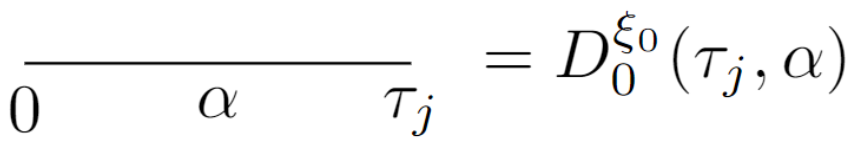
\includegraphics[height=24pt]{images/feynman1.png}

  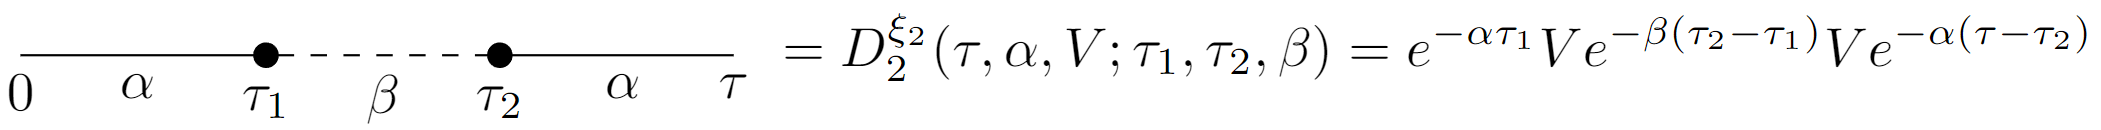
\includegraphics[height=24pt]{images/feynman2.png}
\end{figure}
How can we sample from this function?
\end{frame}

\begin{frame}[containsverbatim]{Diagrammatic Monte Carlo - Task}
  We use the \alert{Metropolis-Hastings algorithm} again, using the diagrams as 
  weights. For ergodicity, we need to implement the following updates:
  \begin{itemize}
    \item Change of $\tau$
    \item Increasing the order of the diagram
    \item Decreasing the order of the diagram
    \item (Change of $\alpha$)
  \end{itemize}
Mind the context factors of the updates when changing the order of the diagram\supercitepage[ch. 12.3.1.2]{fehske}:
\begin{equation*}
  A_{0 \rightarrow 2}=\min \left\{1, \frac{p_{\text {rem }}}{p_{\text {add }}} \frac{D_2^{\xi_2}\left(\tau, \alpha, V ; \tau_1, \tau_2, \beta\right) d \tau_1 d \tau_2}{D_0^{\xi_0}\left(\tau_0, \alpha_0\right) p_1\left(\tau_1\right) p_2\left(\tau_2\right) p_3(\beta) d \tau_1 d \tau_2}\right\}
\end{equation*}
We implement a Python class to sample, analyse and plot the results of the DMC algorithm.
We will first take a look at some of the methods of this class, then have a look at the
whole class \textbf{DMC.py} and finally look at the results.
\end{frame}

\begin{frame}[containsverbatim]{Diagrammatic Monte Carlo Implementation - Initialization}
  \begin{minted}
    [
      baselinestretch=1.2,
      bgcolor=LightGray,
      fontsize=\scriptsize,
      linenos
      ]
      {python}
def __init__(...) -> None:
  # check parameters
  if tau_max <= tau_min:
      raise ValueError("tau_max must be greater than tau_min")
  # And so on...
  self.rng = np.random.default_rng() # set up random number generator
  self.uni = lambda a, b: self.rng.random() * (b - a) + a
  self.n_equ, n_sam, tau_min; tau_max, V, use_change_alpha = ... # Set up config parameters
  self.tau, alpha, beta, tau1, tau2 = ... # Set up state variables
  self.n_tau_acc, n_tau_rej, n_alpha_acc, n_alpha_rej... = 0 # Counters
  self.samples = np.zeros((n_sam, 2) if use_change_alpha else n_sam) # Set up sample array
  # Set up updater methods
  self.updaters = [self.change_tau]
  if use_change_alpha:
      self.updaters.append(self.change_alpha)
  # And so on...

    \end{minted}
  \end{frame}
\begin{frame}[containsverbatim]{Diagrammatic Monte Carlo Implementation - Weight Calculation}
  \begin{minted}
    [
      baselinestretch=1.2,
      bgcolor=LightGray,
      fontsize=\scriptsize,
      linenos
      ]
      {python}
def weight(self, tau=None, alpha=None, beta=None, tau1=None, tau2=None) -> float:
    if tau is None:
        tau = self.tau
    # Same for alpha, beta, tau1 and tau2
    # ...
    # If the diagram is of zero order, the weight is simple
    if beta == 0:
        return np.exp(-alpha * tau)
    # If the diagram is of second order, we need to include
    # two interaction vertices and the beta propagator
    return (
        np.exp(-alpha * tau1)
        * self.V
        * np.exp(-beta * (tau2 - tau1))
        * self.V
        * np.exp(-alpha * (tau - tau2))
    )
  \end{minted}
  As we will see, this method is used in every update to calculate the acceptance ratio.
    \end{frame}

\begin{frame}[containsverbatim]{Diagrammatic Monte Carlo Implementation - Change-$\tau$\&$\alpha$}
  \begin{minted}
    [
      baselinestretch=1.2,
      bgcolor=LightGray,
      fontsize=\scriptsize,
      linenos
      ]
      {python}
def change_tau(self) -> bool:
    prop_tau = self.uni(self.tau2, self.tau_max)
    M = self.weight(tau=prop_tau) / self.weight()
    if M > self.rng.random():
        self.tau = prop_tau
        self.n_tau_acc += 1
        return True
    else:
        self.n_tau_rej += 1
        return False

def change_alpha(self) -> bool:
    prop_alpha = [0.5, 1][int(self.rng.random() * 2)]
    M = self.weight(alpha=prop_alpha) / self.weight()
    if M > self.rng.random():
        self.alpha = prop_alpha
        self.n_alpha_acc += 1
        return True
    else:
        self.n_alpha_rej += 1
        return False
  \end{minted}
\end{frame}

\begin{frame}[containsverbatim]{Diagrammatic Monte Carlo Implementation - Change-Order}
  \begin{minted}
    [
      baselinestretch=1.2,
      bgcolor=LightGray,
      fontsize=\scriptsize,
      linenos
      ]
      {python}
def add_beta(self) -> bool:
    if self.beta != 0:
        self.n_beta_rej += 1
        return False
    prop_tau2 = self.uni(self.tau_min, self.tau)
    prop_tau1 = self.uni(self.tau_min, prop_tau2)
    prop_beta = [0.25, 0.75][int(self.rng.random() * 2)]
    M = self.weight(beta=prop_beta, tau1=prop_tau1, tau2=prop_tau2) / (
        self.weight() / (self.tau - self.tau_min) / (prop_tau2 - self.tau_min) * 0.5
    )
    if M > self.rng.random():
        self.beta = prop_beta
        self.tau1 = prop_tau1
        self.tau2 = prop_tau2
        self.n_beta_acc += 1
        return True
    else:
        self.n_beta_rej += 1
        return False
  \end{minted}
  The remove-$\beta$ update works the same way. The Metropolis ratio is the
  inverse of the add-$\beta$ ratio.
\end{frame}

\begin{frame}[containsverbatim]{Diagrammatic Monte Carlo Implementation - Updating, Sampling}
  \begin{minted}
    [
      baselinestretch=1.2,
      bgcolor=LightGray,
      fontsize=\scriptsize,
      linenos
      ]
      {python}
def update(self) -> bool:
    updater = self.updaters[int(self.rng.random() * len(self.updaters))] 
    return updater()

def sample(self) -> None:
    for i in trange(self.n_sam):
        self.update()
        if self.use_change_alpha:
            self.samples[i, 0] = self.tau
            self.samples[i, 1] = self.alpha
            if self.beta == 0:
                self.n_zero_order[self.alpha] = self.n_zero_order.get(self.alpha, 0) + 1  
        else:
            self.samples[i] = self.tau
            if self.beta == 0:
                self.n_zero_order += 1  
    # Logging ...
  \end{minted}
  Equilibration works the same way, but without sampling.
\end{frame}

\begin{frame}[containsverbatim]{Diagrammatic Monte Carlo Implementation - Normalization}
The normalization constant could still be calculated analytically, but normally this 
is not possible. \\
\alert{Solution}: Use normalization constant $C_0$ of zero order diagram and 
number of zero order diagrams $N_0$ to estimate $C$ \supercitepage[ch. 3.3]{ragni}:
\begin{equation*}
  C\approx C_0\frac{N}{N_0}
\end{equation*}
This is implemented as an alternative to the analytical normalization. Furthermore,
helper methods for plotting and analysis are implemented.\\
\\
Let's take a look at the whole class \textbf{DMC.py}, before we come back to the results.


\end{frame}

\begin{frame}[standout]
  Switching to VS Code
\end{frame}

\begin{frame}[containsverbatim]{Diagrammatic Monte Carlo - Results}
  \begin{columns}
    \column{0.33\linewidth}
      \begin{minted}
        [
          baselinestretch=1.2,
          bgcolor=LightGray,
          fontsize=\scriptsize,
          linenos
          ]
          {python}
from DMC import DMC
dmc = DMC(
    n_equ=int(1e4),
    n_sam=int(5e6),
    tau_min=0,
    tau_max=5,
    alpha_0=1,
    tau_0=1,
    use_change_alpha=True,
    use_change_beta=False,
    use_analytical=True,
)
dmc.equilibrate()
dmc.sample()
dmc.print_I1(0.5)
dmc.print_I1(1)
dmc.print_I2(0.5)
dmc.print_I2(1)
dmc.plot_hist(1)
dmc.plot_hist(0.5)
      \end{minted}
    \column{0.67\linewidth}
    \begin{minted}
      [
        baselinestretch=1.2,
        bgcolor=LightGray,
        fontsize=\scriptsize,
        linenos
        ]
        {python}
Warming up: 10000 steps
Warmup complete: τ acc. ratio of 0.54, α acc. ratio of 0.86
Sampling: 5000000 steps
100%|██████████| 5000000/5000000 [00:25<00:00, 194393.91it/s]
Sampling complete: τ acc. ratio of 0.54, α acc. ratio of 0.85
I1(α=0.5) mean: 2.85430, var: 9.53e-06
I1(α=1) mean: 0.96035, var: 2.40e-06
I2(α=0.5) mean: 7.31758, var: 1.63e-04
I2(α=1) mean: 1.75439, var: 2.34e-05
  \end{minted}
Plots are shown on the next slide.
  \end{columns} 
\end{frame}

\begin{frame}[containsverbatim]{Diagrammatic Monte Carlo - Results}
  \begin{columns}
    \column{0.5\linewidth}
    \begin{figure}
      \centering
      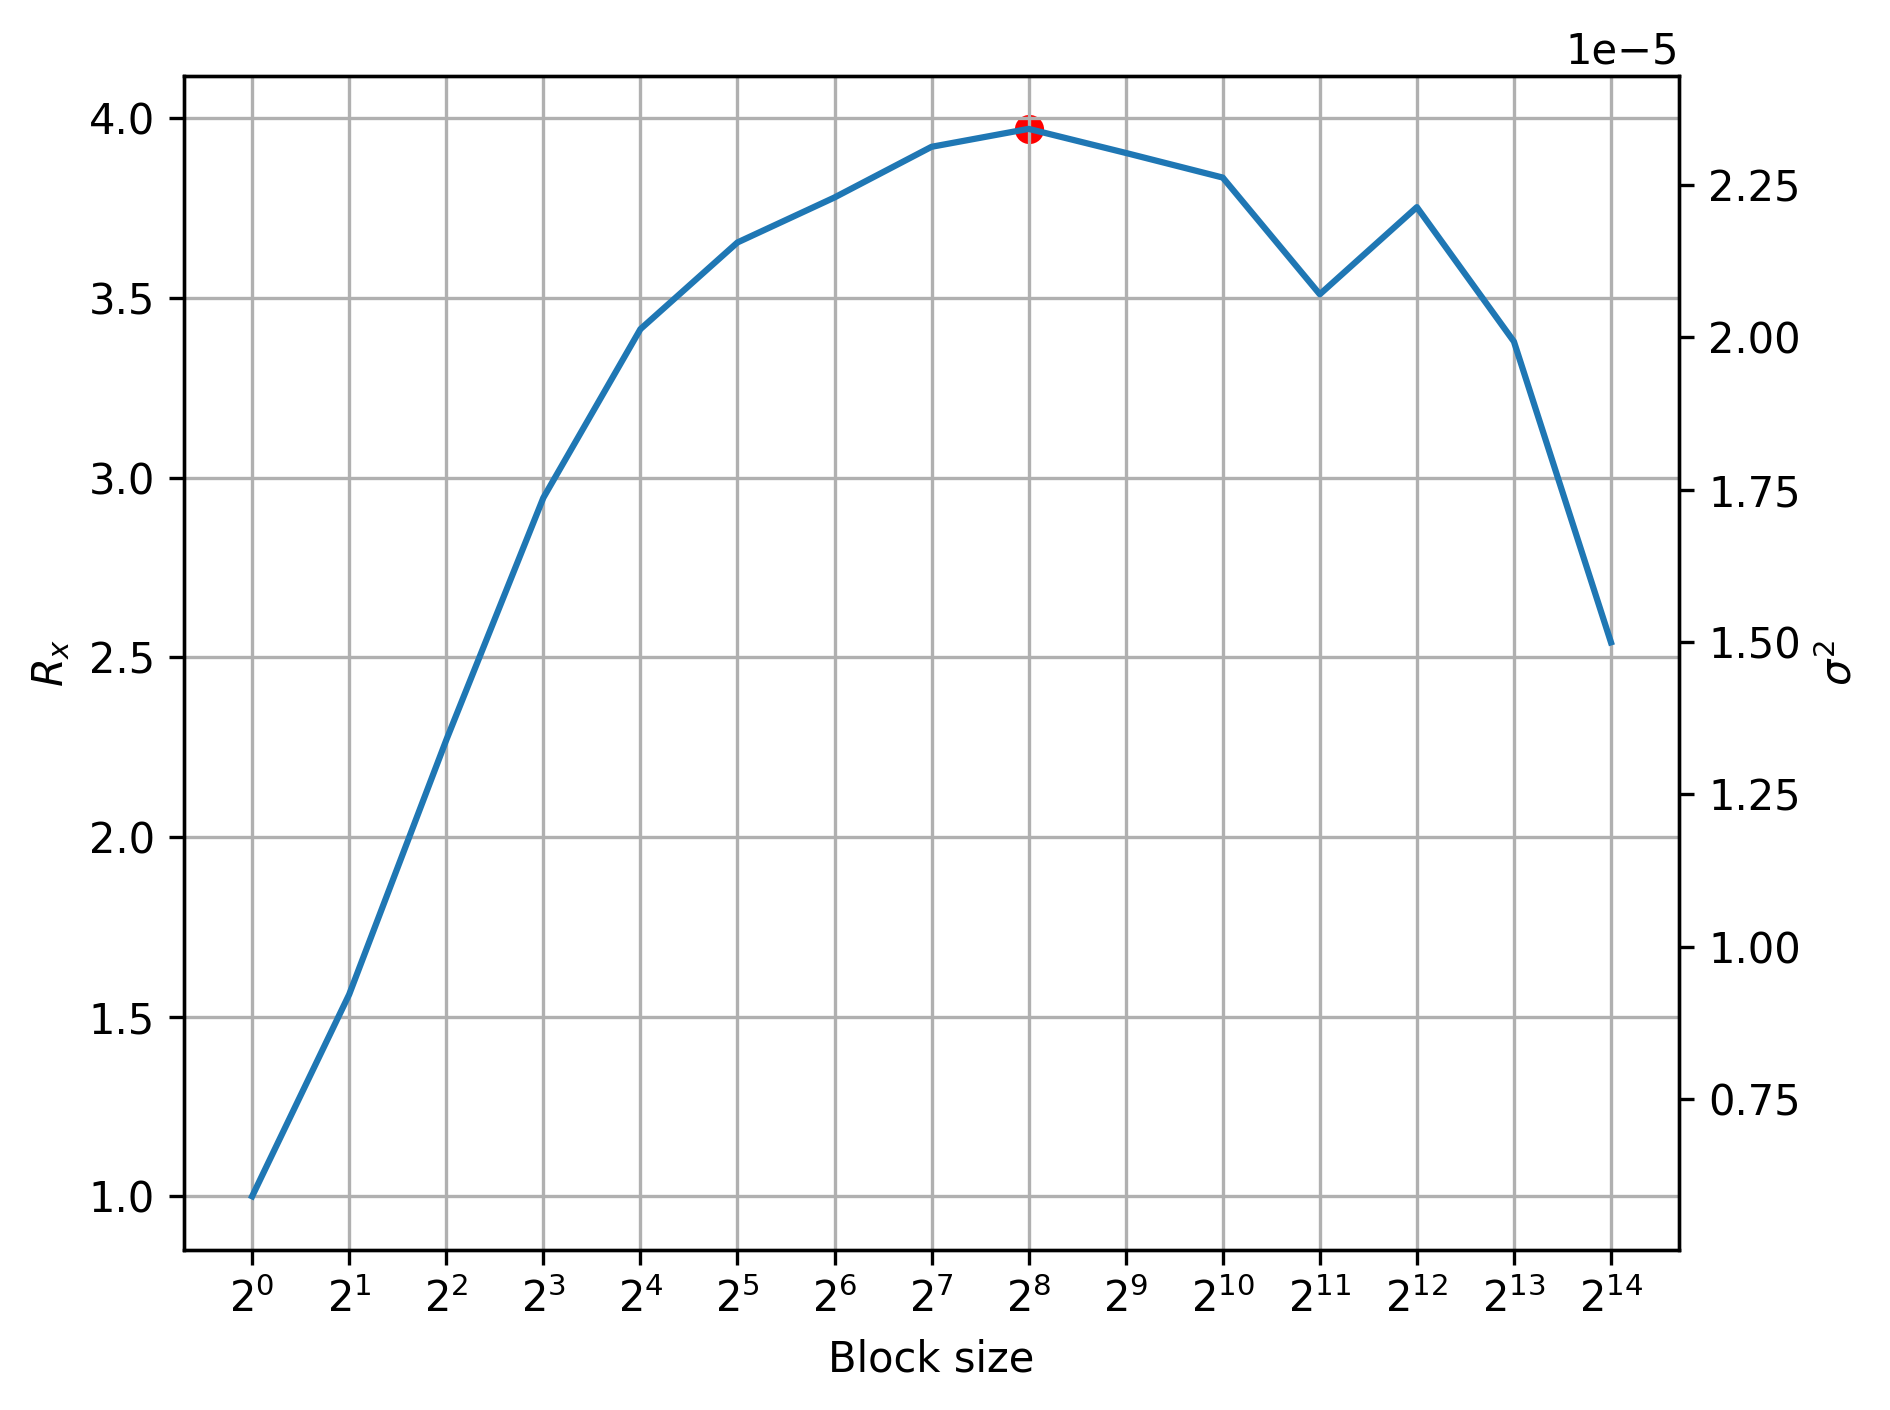
\includegraphics[width=\linewidth]{images/dmc_zero_order_1_i2_blocking.png}
      \caption*{One of the blocking analysis plots}
    \end{figure}
    
    \column{0.5\linewidth}
    \begin{figure}
      \centering
      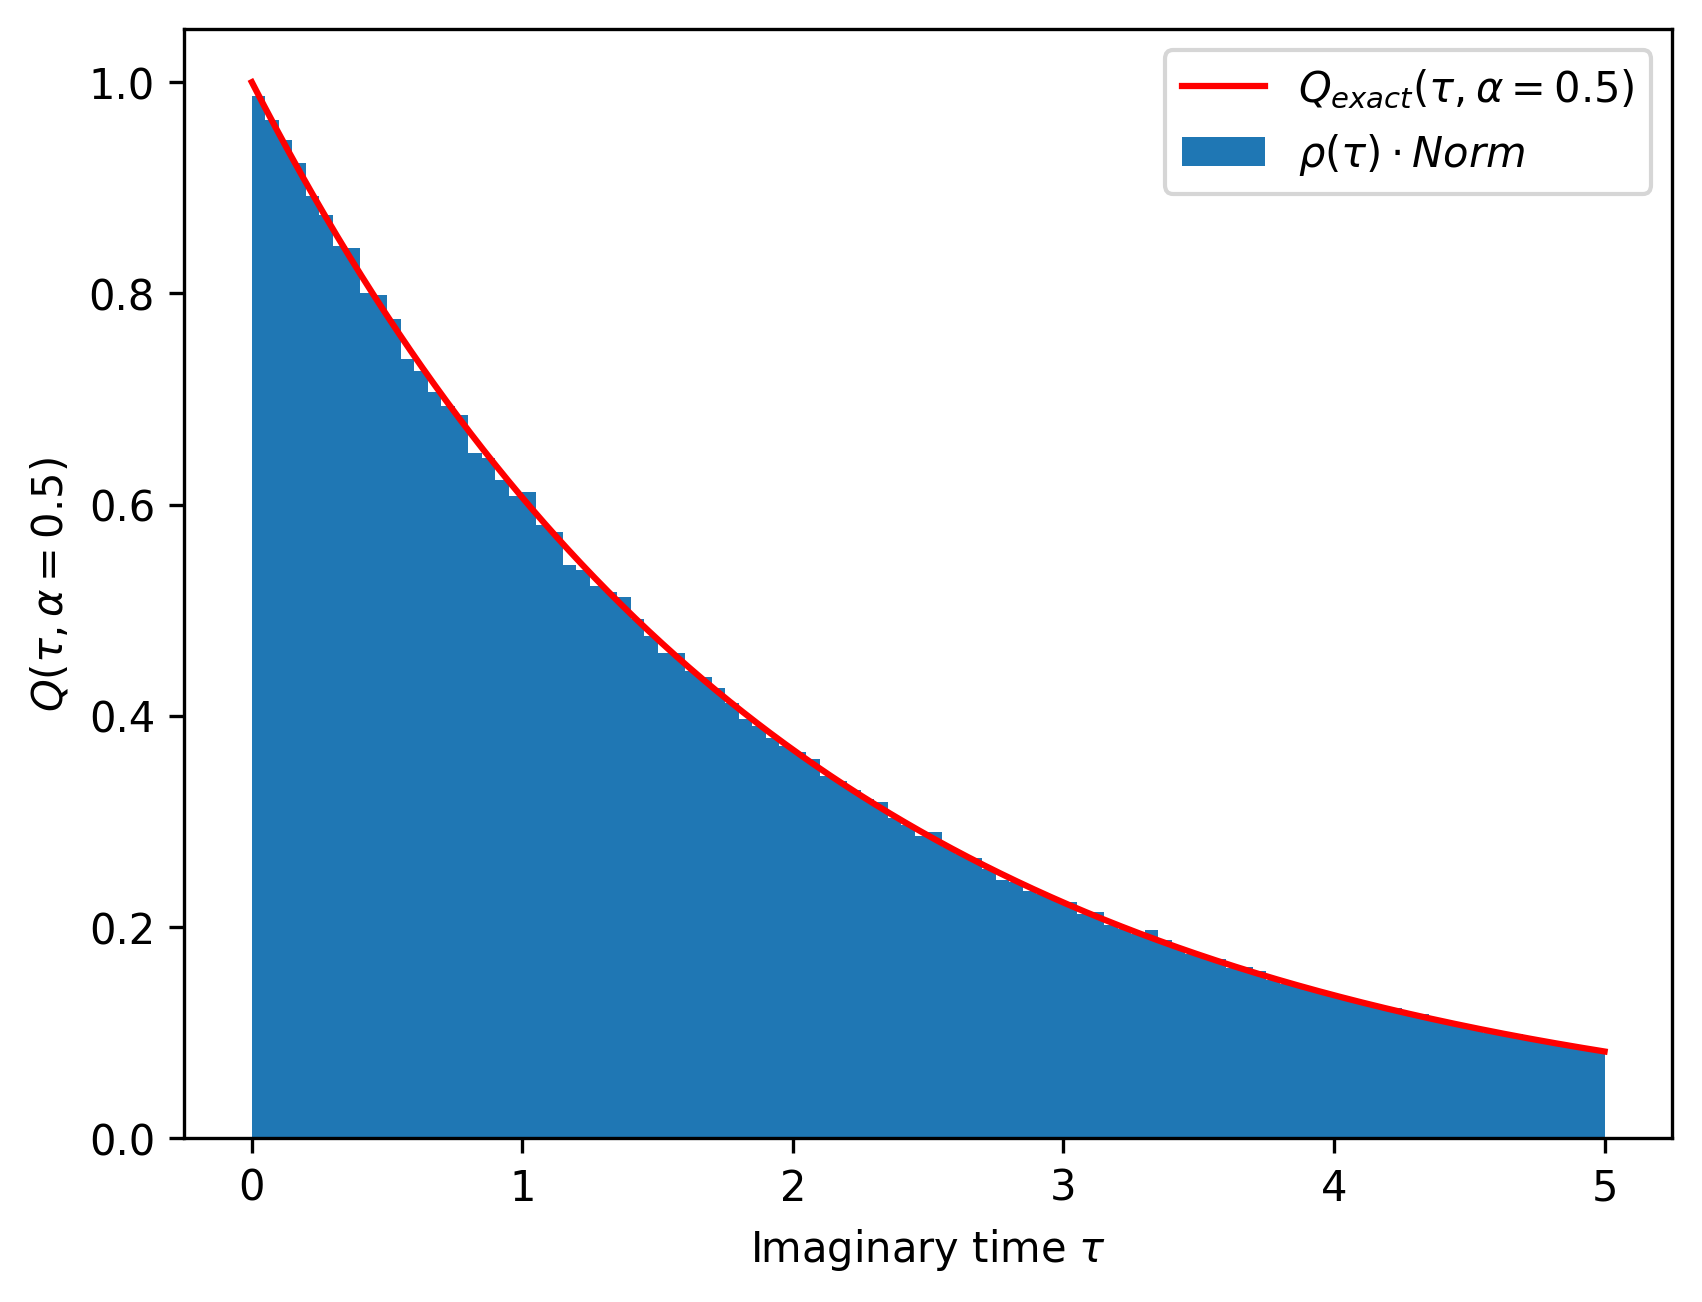
\includegraphics[width=\linewidth]{images/dmc_zero_order_05_hist.png}
      \caption*{Histogram for $\alpha=0.5$}
    \end{figure}
  \end{columns}
\end{frame}


\begin{frame}[containsverbatim]{Diagrammatic Monte Carlo - Results}
  \begin{columns}
    \column{0.33\linewidth}
      \begin{minted}
        [
          baselinestretch=1.2,
          bgcolor=LightGray,
          fontsize=\scriptsize,
          linenos
          ]
          {python}
from DMC import DMC

dmc = DMC(
    n_equ=int(1e4),
    n_sam=int(3e6),
    tau_min=0,
    tau_max=5,
    alpha_0=0.4,
    tau_0=1,
    V=0.5,
    use_change_alpha=False,
    use_change_beta=True,
    use_analytical=True,
)
dmc.equilibrate()
dmc.sample()
dmc.plot_hist()
      \end{minted}
    \column{0.67\linewidth}
    \begin{minted}
      [
        baselinestretch=1.2,
        bgcolor=LightGray,
        fontsize=\scriptsize,
        linenos
        ]
        {python}
Warming up: 10000 steps
Warmup complete: τ acc. ratio of 0.76, β acc. ratio of 0.22
Sampling: 3000000 steps
100%|██████████| 3000000/3000000 [00:14<00:00, 205720.34it/s]
Sampling complete: τ acc. ratio of 0.76, β acc. ratio of 0.22
  \end{minted}
\begin{figure}
  \centering
  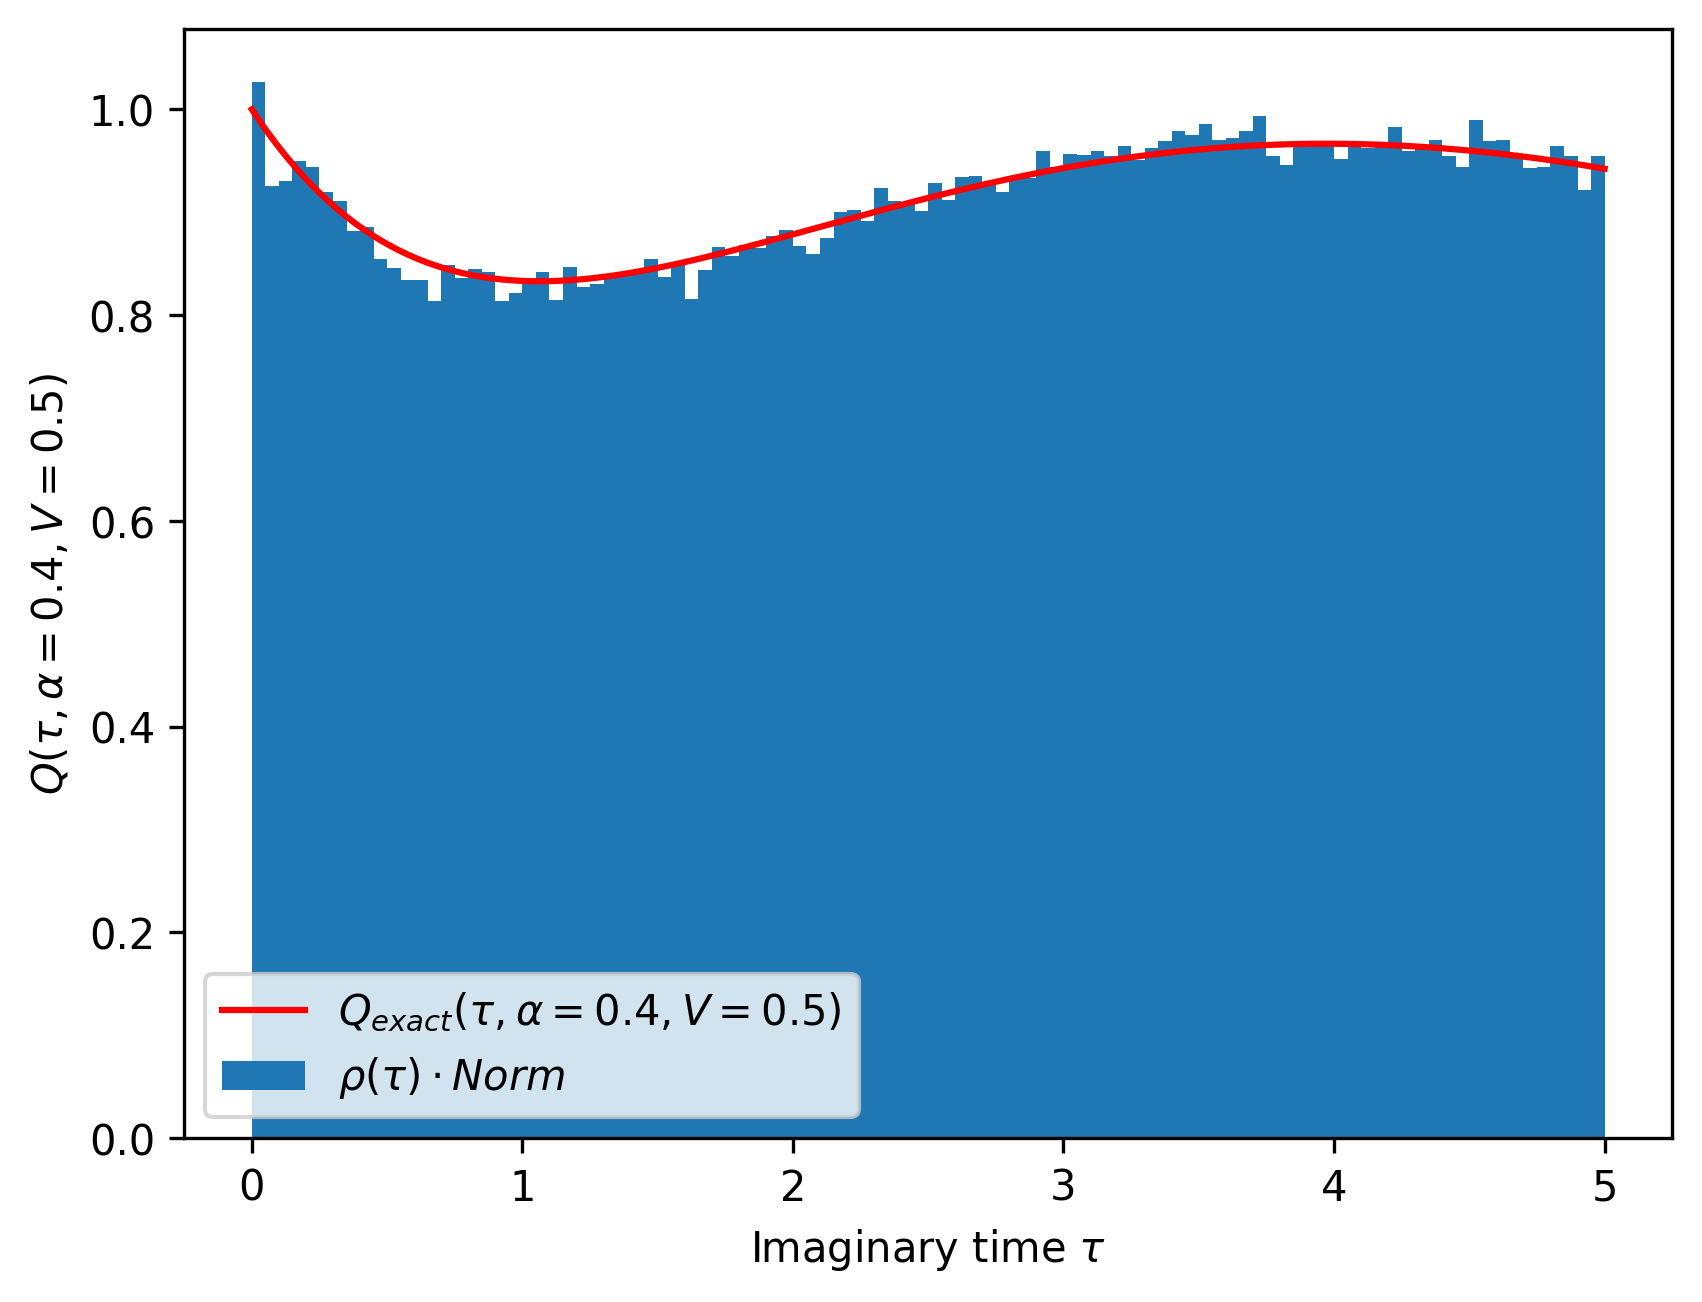
\includegraphics[width=0.7\linewidth]{images/dmc_second_order.png}
\end{figure}
  \end{columns} 
\end{frame}

\section{Task 6: DMC - Green Function Estimator}
\begin{frame}[containsverbatim]{Diagrammatic Monte Carlo - Greens Function Estimator}
  An exact MC estimator for the Greens function can be derived \cite[ch. III.C]{mishchenko}:
  \begin{align*}
    \left\langle q_{\tau_0}\right\rangle_{M C}&=C * Q\left(\tau_0, \alpha, V\right)\\
    q_{\tau_0}(\nu, \tau)&= \begin{cases}q(\nu) \mathcal{D}_\nu\left(\tau_0\right) / \mathcal{D}_\nu(\tau)=\lvert \Gamma_0\rvert^{-1} e^{-\alpha\left(\tau_0-\tau\right)}, & \text { if } \tau \in \Gamma_0 \text { and } \mathcal{D}_\nu(\tau) \neq 0 \\ 0, & \text { otherwise. }\end{cases}
    \end{align*}
    Where I choose $\Gamma_0 = [\tau_0-a, \tau_0+a]$ with $a=\min(0.2,\tau_0,\tau_{\max}-\tau_0)$ \\
    This eliminates the discretization error of the histogram method.\\
    \begin{minted}
      [
        baselinestretch=1.2,
        bgcolor=LightGray,
        fontsize=\scriptsize,
        linenos
        ]
        {python}
def green_estimator(self, tau0: float, alpha: float | None = None) -> float:
    if alpha is None:
        alpha = self.alpha
    tau = self.get_samples(alpha)
    diff = np.subtract.outer(tau0, tau)
    tau0_stacked = np.repeat(tau0, tau.size).reshape(diff.shape)
    mins = np.minimum(np.minimum(tau0_stacked, self.tau_max - tau0_stacked), 0.2)
    res = np.exp(-alpha * (diff)) / (2 * mins)
    res[np.abs(diff) > mins] = 0
    meaned = np.mean(res, axis=1) *self.norm(alpha, analytical=self.use_analytical)
    return meaned
    \end{minted}
\end{frame} 

\begin{frame}[containsverbatim]{Diagrammatic Monte Carlo - Greens Function Estimator - Results}
  Plot of the Greens function estimator for $n=3 \cdot 10^6$ samples:
  \begin{figure}
    \centering
    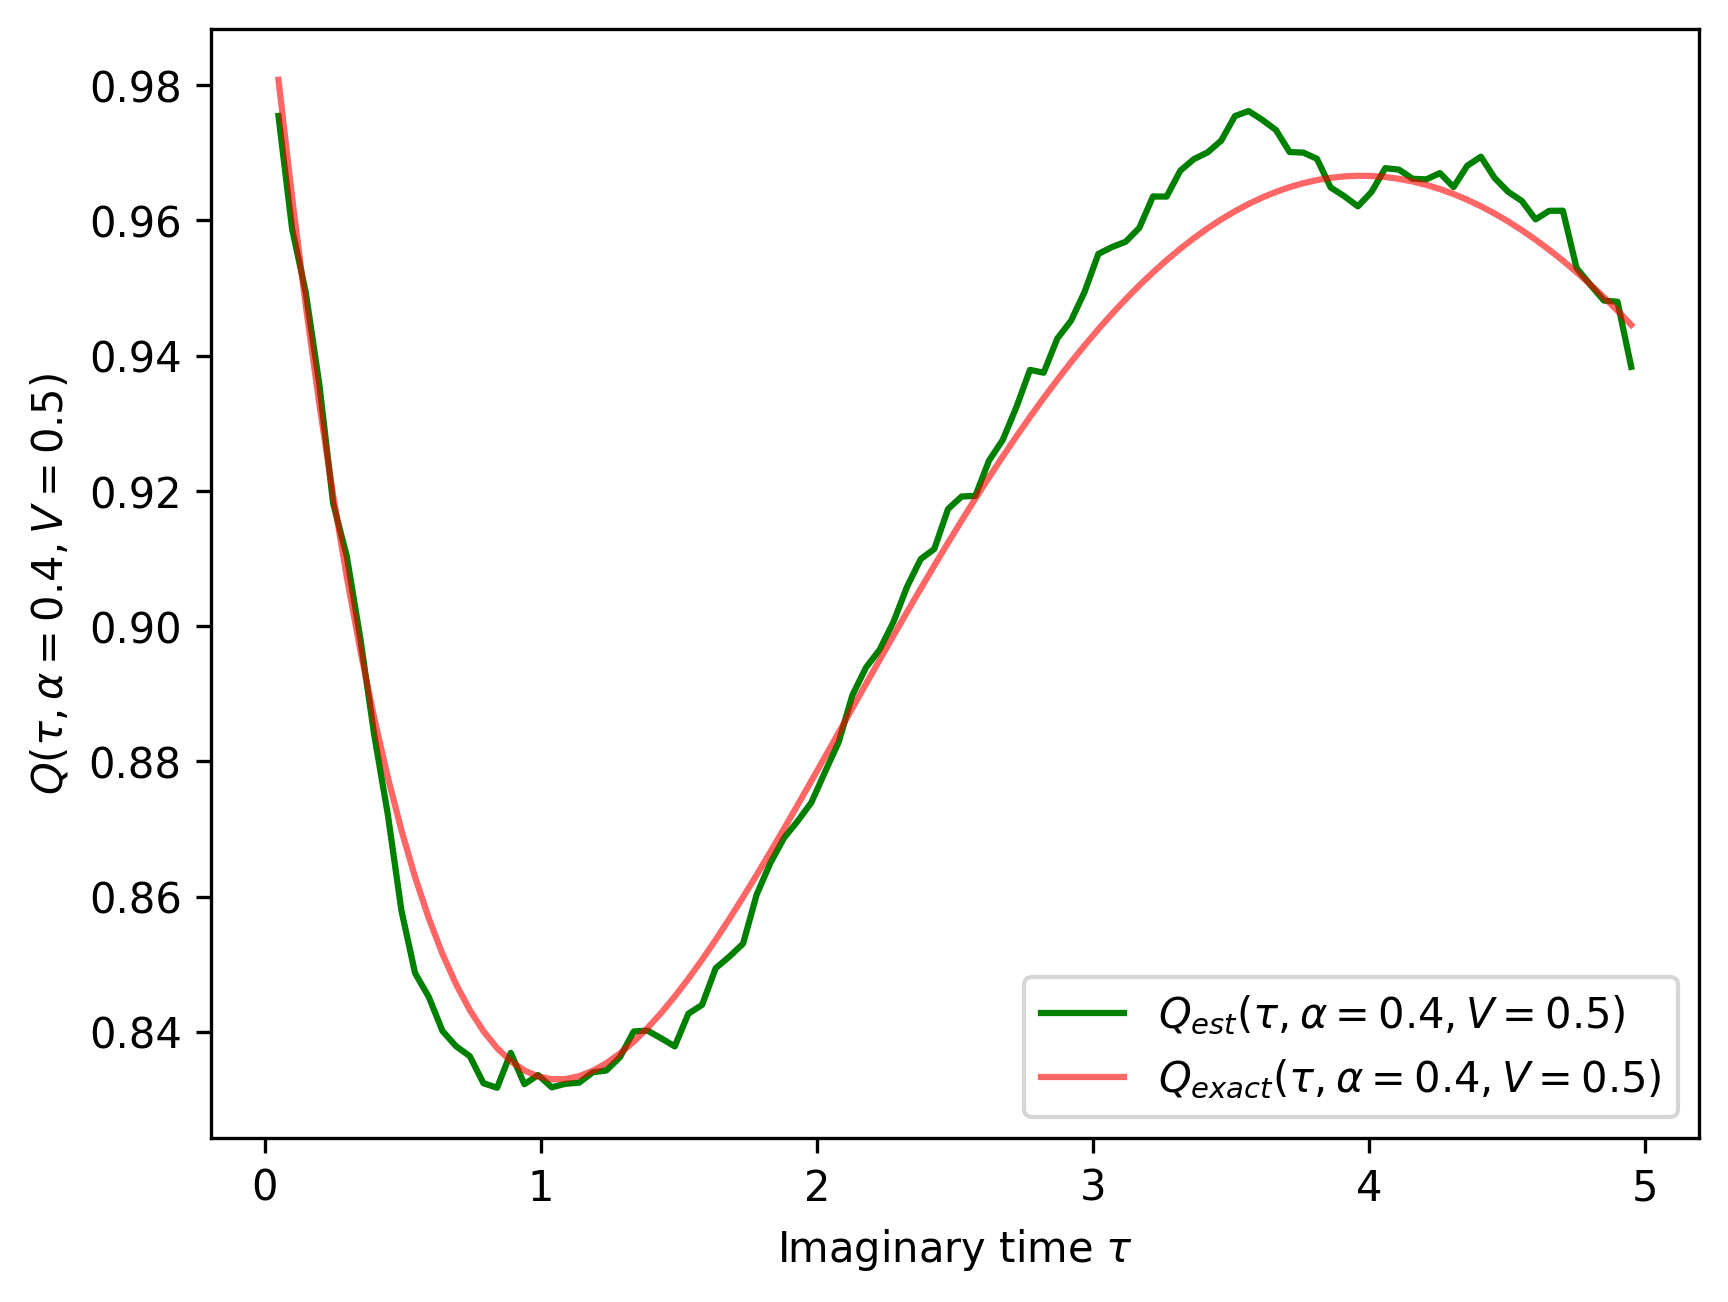
\includegraphics[width=0.65\linewidth]{images/dmc_green_estimator.png}
  \end{figure}
\end{frame}



\renewcommand\appendixname{Appendix}
\appendix


\defbeamertemplate*{bibliography item}{}
{\insertbiblabel}

\begin{frame}[allowframebreaks]{References}
  \bibliographystyle{alpha}
  \bibliography{DMC}
\end{frame}

\end{document}
